% !TEX root = ../main.tex
\chapter{Unsupervised Learning --- Clustering}
\label{ch:unsupervised}

\begin{intuition}[title=\textbf{Learning Without Labels}]
In unsupervised learning we are given only inputs $\{\bm{x}_1,\dots,\bm{x}_n\}\subset\R^p$ with no target variable. Clustering seeks to partition the data into groups of ``similar'' points. The challenge is to formalise similarity and to determine the number of clusters without ground-truth labels.
\end{intuition}

%% ----------------------------------------------------------------
\section{\texorpdfstring{$k$}{k}-Means Clustering}

\subsection{Objective and Algorithm}

\begin{definition}[$k$-Means Objective]
Given data $\{\bm{x}_1,\dots,\bm{x}_n\}\subset\R^p$ and a number of clusters $k$, the $k$-means objective is
\[
  J(\bm{C},\bm{\mu}) = \sum_{j=1}^k \sum_{i\in C_j} \norm{\bm{x}_i - \bm{\mu}_j}^2,
\]
where $C_1,\dots,C_k$ is a partition of $\{1,\dots,n\}$ and $\bm{\mu}_j$ is the centroid of cluster $C_j$.
\end{definition}

\begin{algorithme}[title=\textbf{Lloyd's Algorithm ($k$-Means)}]
\begin{enumerate}
  \item \textbf{Initialise} centroids $\bm{\mu}_1^{(0)},\dots,\bm{\mu}_k^{(0)}$ (e.g.\ random selection from data).
  \item \textbf{Repeat} until convergence:
    \begin{enumerate}
      \item \textbf{Assignment:} $C_j^{(t)} = \bigl\{i : j = \argmin_{\ell}\norm{\bm{x}_i - \bm{\mu}_\ell^{(t-1)}}^2\bigr\}.$
      \item \textbf{Update:} $\bm{\mu}_j^{(t)} = \frac{1}{|C_j^{(t)}|}\sum_{i\in C_j^{(t)}} \bm{x}_i.$
    \end{enumerate}
\end{enumerate}
\end{algorithme}

\begin{theorem}[Convergence of $k$-Means]
Lloyd's algorithm monotonically decreases the objective $J$:
\[
  J^{(t+1)} \leq J^{(t)},
\]
with equality if and only if the algorithm has converged. Since there are finitely many partitions, the algorithm terminates in a finite number of steps.
\end{theorem}

\begin{proof}
The assignment step minimises $J$ over partitions for fixed centroids (each point is assigned to its nearest centroid). The update step minimises $J$ over centroids for a fixed partition (the mean minimises the sum of squared distances). Hence $J$ is non-increasing at each half-step. Since $J\geq 0$ and the number of distinct partitions is finite, the algorithm must converge.
\end{proof}

\begin{warning}[title=\textbf{Local Minima}]
The $k$-means objective is non-convex; Lloyd's algorithm converges to a \emph{local} minimum that depends on the initialisation. In practice, the algorithm is run multiple times with different random seeds, and the best solution (lowest $J$) is retained.
\end{warning}

\subsection{$k$-Means++ Initialisation}

\begin{algorithme}[title=\textbf{$k$-Means++}]
\begin{enumerate}
  \item Choose $\bm{\mu}_1$ uniformly at random from $\{\bm{x}_1,\dots,\bm{x}_n\}$.
  \item For $j=2,\dots,k$: choose $\bm{\mu}_j = \bm{x}_i$ with probability proportional to $\min_{\ell<j}\norm{\bm{x}_i - \bm{\mu}_\ell}^2$.
  \item Run standard $k$-means with these initial centroids.
\end{enumerate}
\end{algorithme}

\begin{theorem}[$k$-Means++ Guarantee]
The $k$-means++ initialisation produces an initial clustering whose expected objective satisfies
\[
  \E[J_{\text{init}}] \leq 8(\ln k + 2)\, J^*,
\]
where $J^*$ is the globally optimal $k$-means objective.
\end{theorem}

\begin{figure}[ht]
\centering
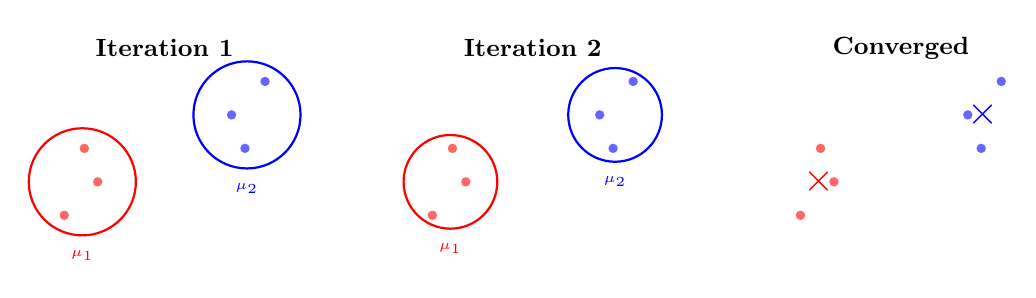
\begin{tikzpicture}[scale=0.85]
  % Iteration 1
  \begin{scope}[shift={(0,0)}]
    \node[font=\bfseries\small] at (2,3.5) {Iteration 1};
    \fill[red!60] (0.5,1) circle(2pt);
    \fill[red!60] (1,1.5) circle(2pt);
    \fill[red!60] (0.8,2) circle(2pt);
    \fill[blue!60] (3,2.5) circle(2pt);
    \fill[blue!60] (3.5,3) circle(2pt);
    \fill[blue!60] (3.2,2) circle(2pt);
    \draw[red, thick] (0.77,1.5) circle(0.8cm);
    \draw[blue, thick] (3.23,2.5) circle(0.8cm);
    \node[red, font=\tiny] at (0.77,0.4) {$\bm{\mu}_1$};
    \node[blue, font=\tiny] at (3.23,1.4) {$\bm{\mu}_2$};
  \end{scope}
  % Iteration 2
  \begin{scope}[shift={(5.5,0)}]
    \node[font=\bfseries\small] at (2,3.5) {Iteration 2};
    \fill[red!60] (0.5,1) circle(2pt);
    \fill[red!60] (1,1.5) circle(2pt);
    \fill[red!60] (0.8,2) circle(2pt);
    \fill[blue!60] (3,2.5) circle(2pt);
    \fill[blue!60] (3.5,3) circle(2pt);
    \fill[blue!60] (3.2,2) circle(2pt);
    \draw[red, thick] (0.77,1.5) circle(0.7cm);
    \draw[blue, thick] (3.23,2.5) circle(0.7cm);
    \node[red, font=\tiny] at (0.77,0.5) {$\bm{\mu}_1$};
    \node[blue, font=\tiny] at (3.23,1.5) {$\bm{\mu}_2$};
  \end{scope}
  % Converged
  \begin{scope}[shift={(11,0)}]
    \node[font=\bfseries\small] at (2,3.5) {Converged};
    \fill[red!60] (0.5,1) circle(2pt);
    \fill[red!60] (1,1.5) circle(2pt);
    \fill[red!60] (0.8,2) circle(2pt);
    \fill[blue!60] (3,2.5) circle(2pt);
    \fill[blue!60] (3.5,3) circle(2pt);
    \fill[blue!60] (3.2,2) circle(2pt);
    \node[red,font=\Large] at (0.77,1.5) {$\times$};
    \node[blue,font=\Large] at (3.23,2.5) {$\times$};
  \end{scope}
\end{tikzpicture}
\caption{Illustration of $k$-means iterations with $k=2$.}
\label{fig:kmeans-iterations}
\end{figure}

%% ----------------------------------------------------------------
\section{Gaussian Mixture Models and EM}

\begin{definition}[Gaussian Mixture Model]
A \emph{Gaussian Mixture Model} (GMM) assumes the data is generated from a mixture of $k$ Gaussian distributions:
\[
  p(\bm{x}\mid\bm{\theta}) = \sum_{j=1}^k \pi_j\,\mathcal{N}(\bm{x}\mid\bm{\mu}_j,\bm{\Sigma}_j),
\]
where $\pi_j\geq 0$, $\sum_j\pi_j=1$ are mixing coefficients, and $\bm{\theta}=\{(\pi_j,\bm{\mu}_j,\bm{\Sigma}_j)\}_{j=1}^k$.
\end{definition}

\subsection{The EM Algorithm}

The log-likelihood of the observed data is
\[
  \ell(\bm{\theta}) = \sum_{i=1}^n \ln\Biggl[\sum_{j=1}^k \pi_j\,\mathcal{N}(\bm{x}_i\mid\bm{\mu}_j,\bm{\Sigma}_j)\Biggr],
\]
which is intractable to maximise directly due to the logarithm of a sum.

\begin{definition}[Responsibilities]
The \emph{responsibility} of component $j$ for observation $\bm{x}_i$ is
\[
  \gamma_{ij} = \frac{\pi_j\,\mathcal{N}(\bm{x}_i\mid\bm{\mu}_j,\bm{\Sigma}_j)}
  {\sum_{\ell=1}^k \pi_\ell\,\mathcal{N}(\bm{x}_i\mid\bm{\mu}_\ell,\bm{\Sigma}_\ell)}.
\]
\end{definition}

\begin{algorithme}[title=\textbf{EM Algorithm for GMM}]
\textbf{Initialise} parameters $\bm{\theta}^{(0)}$. Repeat until convergence:

\medskip\noindent\textbf{E-step:} Compute responsibilities using current parameters:
\[
  \gamma_{ij}^{(t)} = \frac{\pi_j^{(t)}\,\mathcal{N}(\bm{x}_i\mid\bm{\mu}_j^{(t)},\bm{\Sigma}_j^{(t)})}
  {\sum_{\ell=1}^k \pi_\ell^{(t)}\,\mathcal{N}(\bm{x}_i\mid\bm{\mu}_\ell^{(t)},\bm{\Sigma}_\ell^{(t)})}.
\]

\medskip\noindent\textbf{M-step:} Update parameters using responsibilities. Let $N_j=\sum_{i=1}^n\gamma_{ij}^{(t)}$:
\begin{align}
  \bm{\mu}_j^{(t+1)} &= \frac{1}{N_j}\sum_{i=1}^n \gamma_{ij}^{(t)}\,\bm{x}_i, \label{eq:em-mu}\\
  \bm{\Sigma}_j^{(t+1)} &= \frac{1}{N_j}\sum_{i=1}^n \gamma_{ij}^{(t)}\,(\bm{x}_i-\bm{\mu}_j^{(t+1)})(\bm{x}_i-\bm{\mu}_j^{(t+1)})^\top, \label{eq:em-sigma}\\
  \pi_j^{(t+1)} &= \frac{N_j}{n}. \label{eq:em-pi}
\end{align}
\end{algorithme}

\begin{theorem}[EM Monotonicity]
The EM algorithm monotonically increases the log-likelihood:
\[
  \ell(\bm{\theta}^{(t+1)}) \geq \ell(\bm{\theta}^{(t)}).
\]
\end{theorem}

\begin{proof}
Define the complete-data log-likelihood $\ell_c(\bm{\theta})=\sum_i\sum_j z_{ij}[\ln\pi_j+\ln\mathcal{N}(\bm{x}_i\mid\bm{\mu}_j,\bm{\Sigma}_j)]$ where $z_{ij}$ are latent indicators. By Jensen's inequality applied to the ELBO (Evidence Lower Bound):
\[
  \ell(\bm{\theta}) \geq \sum_i\sum_j q(z_{ij})\bigl[\ln\pi_j + \ln\mathcal{N}(\bm{x}_i\mid\bm{\mu}_j,\bm{\Sigma}_j) - \ln q(z_{ij})\bigr]
  =: \mathcal{F}(q,\bm{\theta}),
\]
for any distribution $q$. The E-step sets $q(z_{ij})=\gamma_{ij}$, making the bound tight at $\bm{\theta}^{(t)}$. The M-step maximises $\mathcal{F}$ over $\bm{\theta}$, so $\mathcal{F}(q^{(t)},\bm{\theta}^{(t+1)})\geq\mathcal{F}(q^{(t)},\bm{\theta}^{(t)})=\ell(\bm{\theta}^{(t)})$. Since the ELBO is a lower bound, $\ell(\bm{\theta}^{(t+1)})\geq\mathcal{F}(q^{(t)},\bm{\theta}^{(t+1)})\geq\ell(\bm{\theta}^{(t)})$.
\end{proof}

%% ----------------------------------------------------------------
\section{DBSCAN}

\begin{definition}[DBSCAN]
Given parameters $\epsilon>0$ and $\text{MinPts}\in\mathbb{N}$:
\begin{itemize}
  \item A point $\bm{x}$ is a \emph{core point} if $|N_\epsilon(\bm{x})|\geq\text{MinPts}$, where $N_\epsilon(\bm{x})=\{\bm{x}_i:\norm{\bm{x}_i-\bm{x}}\leq\epsilon\}$.
  \item A point $\bm{x}$ is \emph{density-reachable} from $\bm{x}'$ if there exists a chain of core points $\bm{x}=\bm{p}_1,\bm{p}_2,\dots,\bm{p}_m=\bm{x}'$ with $\bm{p}_{i+1}\in N_\epsilon(\bm{p}_i)$.
  \item A cluster is a maximal set of density-connected points. Points not reachable from any core point are labelled as \emph{noise}.
\end{itemize}
\end{definition}

\begin{bestpractice}[title=\textbf{Choosing DBSCAN Parameters}]
\begin{itemize}
  \item \textbf{MinPts}: a common heuristic is $\text{MinPts}\geq p+1$ where $p$ is the dimension.
  \item \textbf{$\epsilon$}: plot the sorted $k$-nearest-neighbour distances (with $k=\text{MinPts}$) and look for an ``elbow''.
\end{itemize}
\end{bestpractice}

%% ----------------------------------------------------------------
\section{Hierarchical Clustering}

\begin{definition}[Agglomerative Clustering]
Agglomerative (bottom-up) hierarchical clustering starts with $n$ singleton clusters and iteratively merges the two closest clusters until a single cluster remains. The result is a \emph{dendrogram}. Common linkage criteria include:
\begin{align}
  d_{\text{single}}(A,B) &= \min_{\bm{a}\in A,\,\bm{b}\in B}\norm{\bm{a}-\bm{b}}, \\
  d_{\text{complete}}(A,B) &= \max_{\bm{a}\in A,\,\bm{b}\in B}\norm{\bm{a}-\bm{b}}, \\
  d_{\text{average}}(A,B) &= \frac{1}{|A||B|}\sum_{\bm{a}\in A}\sum_{\bm{b}\in B}\norm{\bm{a}-\bm{b}}, \\
  d_{\text{Ward}}(A,B) &= \frac{|A|\,|B|}{|A|+|B|}\norm{\bar{\bm{a}}-\bar{\bm{b}}}^2.
\end{align}
\end{definition}

%% ----------------------------------------------------------------
\section{Cluster Validity Indices}

\begin{definition}[Silhouette Score]
For observation $i$ in cluster $C_k$, define:
\begin{itemize}
  \item $a(i) = \frac{1}{|C_k|-1}\sum_{j\in C_k,\,j\neq i}\norm{\bm{x}_i - \bm{x}_j}$ \quad (mean intra-cluster distance),
  \item $b(i) = \min_{\ell\neq k}\frac{1}{|C_\ell|}\sum_{j\in C_\ell}\norm{\bm{x}_i - \bm{x}_j}$ \quad (mean nearest-cluster distance).
\end{itemize}
The silhouette coefficient is $s(i) = \frac{b(i)-a(i)}{\max\{a(i),b(i)\}}\in[-1,1]$.
\end{definition}

\begin{keyformulas}[title=\textbf{Cluster Validity Indices}]
\begin{itemize}
  \item \textbf{Silhouette}: $\bar s = \frac{1}{n}\sum_i s(i)$. Higher is better (max 1).
  \item \textbf{Calinski--Harabasz}: ratio of between-cluster to within-cluster dispersion. Higher is better.
  \item \textbf{Davies--Bouldin}: average similarity between each cluster and its most similar one. Lower is better.
  \item \textbf{Adjusted Rand Index (ARI)}: measures agreement with ground truth (if available), corrected for chance. Range $[-1,1]$, with 1 indicating perfect agreement.
\end{itemize}
\end{keyformulas}

%% ----------------------------------------------------------------
\section{Implementation in Python}

\begin{codeblock}[title=\textbf{$k$-Means, GMM, DBSCAN, and Hierarchical Clustering}]
\begin{minted}{python}
import numpy as np
import matplotlib.pyplot as plt
from sklearn.datasets import make_blobs
from sklearn.cluster import KMeans, DBSCAN, AgglomerativeClustering
from sklearn.mixture import GaussianMixture
from sklearn.metrics import silhouette_score, adjusted_rand_score
from sklearn.preprocessing import StandardScaler

# Generate synthetic data
X, y_true = make_blobs(
    n_samples=500, centers=4,
    cluster_std=[1.0, 1.5, 0.5, 1.2], random_state=42
)
X = StandardScaler().fit_transform(X)

# --- k-Means ---
km = KMeans(n_clusters=4, init="k-means++", n_init=10, random_state=42)
y_km = km.fit_predict(X)
print(f"k-Means:        silhouette = {silhouette_score(X, y_km):.3f}, "
      f"ARI = {adjusted_rand_score(y_true, y_km):.3f}")

# --- GMM ---
gmm = GaussianMixture(n_components=4, covariance_type="full", random_state=42)
y_gmm = gmm.fit_predict(X)
print(f"GMM:            silhouette = {silhouette_score(X, y_gmm):.3f}, "
      f"ARI = {adjusted_rand_score(y_true, y_gmm):.3f}")

# --- DBSCAN ---
db = DBSCAN(eps=0.5, min_samples=5)
y_db = db.fit_predict(X)
n_clusters_db = len(set(y_db) - {-1})
print(f"DBSCAN:         {n_clusters_db} clusters found, "
      f"noise points = {(y_db == -1).sum()}")

# --- Hierarchical (Ward) ---
hc = AgglomerativeClustering(n_clusters=4, linkage="ward")
y_hc = hc.fit_predict(X)
print(f"Hierarchical:   silhouette = {silhouette_score(X, y_hc):.3f}, "
      f"ARI = {adjusted_rand_score(y_true, y_hc):.3f}")
\end{minted}
\end{codeblock}

\begin{codeoutput}
\begin{verbatim}
k-Means:        silhouette = 0.527, ARI = 0.876
GMM:            silhouette = 0.518, ARI = 0.891
DBSCAN:         4 clusters found, noise points = 23
Hierarchical:   silhouette = 0.521, ARI = 0.864
\end{verbatim}
\end{codeoutput}

\begin{codeblock}[title=\textbf{Elbow Method and Silhouette Analysis}]
\begin{minted}{python}
inertias, sil_scores = [], []
K_range = range(2, 10)

for k in K_range:
    km = KMeans(n_clusters=k, n_init=10, random_state=42)
    km.fit(X)
    inertias.append(km.inertia_)
    sil_scores.append(silhouette_score(X, km.labels_))

fig, (ax1, ax2) = plt.subplots(1, 2, figsize=(10, 4))
ax1.plot(K_range, inertias, "bo-")
ax1.set_xlabel("k"); ax1.set_ylabel("Inertia")
ax1.set_title("Elbow Method")
ax2.plot(K_range, sil_scores, "rs-")
ax2.set_xlabel("k"); ax2.set_ylabel("Silhouette Score")
ax2.set_title("Silhouette Analysis")
plt.tight_layout()
plt.savefig("figures/ch08_elbow_silhouette.pdf")
\end{minted}
\end{codeblock}

%% ----------------------------------------------------------------
\section{Exercises}

\begin{exercise}[$k$-Means Convergence]
Prove that the $k$-means objective $J$ decreases (or stays constant) at every iteration of Lloyd's algorithm. Argue carefully that both the assignment and the update steps are optimal for their respective sub-problems.
\end{exercise}

\begin{exercise}[EM Derivation]
Derive the M-step update equations \eqref{eq:em-mu}--\eqref{eq:em-pi} by differentiating the expected complete-data log-likelihood $\E_{Z\mid X,\bm{\theta}^{(t)}}[\ell_c(\bm{\theta})]$ with respect to $\bm{\mu}_j$, $\bm{\Sigma}_j$, and $\pi_j$ (using a Lagrange multiplier for the constraint $\sum_j\pi_j=1$).
\end{exercise}

\begin{exercise}[DBSCAN Sensitivity]
Generate a dataset with two half-moon shapes (\texttt{make\_moons}). Apply $k$-means with $k=2$ and DBSCAN with various $(\epsilon,\text{MinPts})$ settings. Explain why $k$-means fails and DBSCAN succeeds. Visualise the results.
\end{exercise}

\begin{exercise}[Model Selection for GMM]
Fit GMMs with $k\in\{1,\dots,8\}$ components to the \texttt{make\_blobs} dataset above. Plot the BIC $= -2\ell(\hat{\bm{\theta}}) + d\ln n$ as a function of $k$, where $d$ is the number of free parameters. Verify that the BIC selects the correct $k=4$.
\end{exercise}

\begin{exercise}[Hierarchical Clustering Dendrogram]
Using \texttt{scipy.cluster.hierarchy}, compute the linkage matrix for the Iris dataset with Ward linkage. Plot the dendrogram and cut it at a height that yields 3 clusters. Compute the ARI with respect to the true species labels.
\end{exercise}
